\section{The Book Embedding Problem}\label{section:book-problem}

In this section we first present some basic definitions from graph theory. Then we formally formulate the problem \probBook that we consider in this thesis.

A \emph{graph} $G$ is a pair $(V, E)$ where $V$ is a non-empty finite set and
$E \subseteq \binom{V}{2}$. The set $V$ is called the set of \emph{vertices of~$G$}
and $E$ is the set of \emph{edges of~$G$}. We use $V(G)$ to refer to the vertices
of $G$~and $E(G)$ to refer to the edges of~$G$. A planar embedding of a graph~$G$ is a drawing of~$G$ in~$\SR^2$
such that edges do not intersect except at common endpoints. Planar embeddings are revisited more formally at the start of \myref{ch:preliminaries}.

A page embedding is a special planar embedding.

\begin{definition}
\label{def:page-embed}
A \emph{page embedding} of a graph $G = (V, E)$ is a planar embedding of~$G$ such that
the vertices of $G$ lie on the \emph{real line} $\SR \times \{0\}$ and every edge lies in the \emph{upper half-plane} $\bigl\{(x, y) \in \SR^2\colon y > 0\bigr\}$ apart from the edge's endpoints.
\end{definition}

\begin{figure}[\placement]
	\centering
	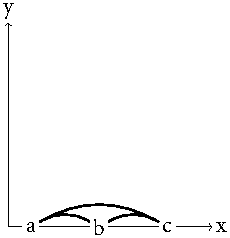
\includegraphics{figures/t_page_c3}
	\caption[Page embedding of $C_3$]{A page embedding of $C_3$}
	\label{figure:page-c3}
\end{figure}

\myref{figure:page-c3} depicts a page embedding for~$C_3$, the cycle on three~vertices.
By taking multiple page embeddings, we get a book embedding. 

\begin{definition}
\label{def:book-embed}
A \emph{book embedding} of graphs $G_1 = (V, E_1),\dotsc,\allowbreak G_k = (V, E_k)$ on the same set of vertices consists of page embeddings for each of the graphs that coincide in their vertex positions. 

In the setting of book embeddings the line $\SR \times \{0\}$
is also called the \emph{spine}. We only demand that edges in the same
graph~$G_i$ do not intersect. This can also be interpreted as giving each graph~$G_i$ its own upper half-plane, which we also call the \emph{page of~$G_i$}. Whenever we refer to a page in this thesis, we usually
mean the graph~$G_i$ on this page.
%The metaphor of an embedding into a book is then justified: The vertices are placed on the real line, the ``spine'' of the book, and the edges on their own copy of the upper half-plane, their ``page'' of the book. 
\end{definition}

The embeddability problem now asks whether such an embedding exists.
\newProb{\probBook}{A vertex set $V$ and edge sets $E_1,\dotsc, E_k \subseteq \binom{V}{2}$}
{Is there a book embedding of $(V, E_1),\dotsc, (V, E_k)$?}


In the literature \emph{book embedding} usually refers to the somewhat different problem \probBookNormal. Instead of directly embedding $k$~graphs
into $k$~pages, we first have to get $k$~graphs by arbitrarily partitioning the edges of a graph into 
$k$~parts and then embed these into $k$~pages. The problem
we call \emph{book embedding} is often called \emph{book embedding with fixed page assignment} in the literature. 
\newProb{\probBookNormal}{A vertex set $V$, an edge set~$E \in \binom{V}{2}$ and a number~$k\geq 1$}
{Is there a partition~$E = \bigcup_{i=1}^{k} E_i$ such that $(V, E_1), \dotsc, (V, E_k)$ is book embeddable?}
We depict this
assignment of the edges to the pages that has already been fixed either by using different colours or in the case of exactly two pages by one set of edges being drawn above and one below the spine.